%%%%%%%%%%%%%%%%%%%%%%%%%%%%%%%%%%%%%%%%%
% kaobook
% LaTeX Template
% Version 1.2 (4/1/2020)
%
% This template originates from:
% https://www.LaTeXTemplates.com
%
% For the latest template development version and to make contributions:
% https://github.com/fmarotta/kaobook
%
% Authors:
% Federico Marotta (federicomarotta@mail.com)
% Based on the doctoral thesis of Ken Arroyo Ohori (https://3d.bk.tudelft.nl/ken/en)
% and on the Tufte-LaTeX class.
% Modified for LaTeX Templates by Vel (vel@latextemplates.com)
%
% License:
% CC0 1.0 Universal (see included MANIFEST.md file)
%
%%%%%%%%%%%%%%%%%%%%%%%%%%%%%%%%%%%%%%%%%

%----------------------------------------------------------------------------------------
%	PACKAGES AND OTHER DOCUMENT CONFIGURATIONS
%----------------------------------------------------------------------------------------

\documentclass[
	fontsize=13pt, % Base font size
	twoside=false, % Use different layouts for even and odd pages (in particular, if twoside=true, the margin column will be always on the outside)
	%open=any, % If twoside=true, uncomment this to force new chapters to start on any page, not only on right (odd) pages
	%chapterprefix=true, % Uncomment to use the word "Chapter" before chapter numbers everywhere they appear
	%chapterentrydots=true, % Uncomment to output dots from the chapter name to the page number in the table of contents
	numbers=noenddot, % Comment to output dots after chapter numbers; the most common values for this option are: enddot, noenddot and auto (see the KOMAScript documentation for an in-depth explanation)
	%draft=true, % If uncommented, rulers will be added in the header and footer
	%overfullrule=true, % If uncommented, overly long lines will be marked by a black box; useful for correcting spacing problems
]{kaobook}
%!TEX root = ../thesis.tex

%\hypersetup{colorlinks,linktocpage,urlcolor=red}
%
%\definecolor{myGreen}{HTML}{05C18E} 
%\definecolor{myGreenDarker}{HTML}{178C6C} \colorlet{mylinkcolor}{green!50!black}

\definecolor{webbrown}{rgb}{.6,0,0}

\hypersetup{
  colorlinks=true,
  linkcolor=black, %myGreenDarker
%  urlcolor=myGreenDarker,
  citecolor = webbrown,
  urlcolor=webbrown,
  hyperfootnotes=false,
  hypertexnames,
  bookmarks=true}
  
%\setsidenotefont{\color{black}\footnotesize}   <-- set the color and font here
%\setmarginnotefont{\color{black}\footnotesize} <-- and here
%
%\renewcommand{\maketitlepage}[0]{%
%  \cleardoublepage%
%  {%
%  \sffamily%
%  \begin{fullwidth}%
%  \fontsize{18}{20}\selectfont\par\noindent\textcolor{darkgray}{\allcaps{\thanklessauthor}}%
%  \vspace{11.5pc}%
%  \fontsize{24}{45}\selectfont\par\noindent\textcolor{darkgray}{\allcaps{\thanklesstitle}}
%  \fontsize{17.4}{25}\selectfont\par\noindent\textcolor{darkgray}{\allcaps{For Affective Touch Communication}}%
%  \fontsize{10.0}{17}\selectfont\par\noindent\textcolor{Gray}{\allcaps{Devices that touch to convey emotions and feel that contact}}%
%
%  \vfill%
%  \fontsize{14}{16}\selectfont\par\noindent\allcaps{\thanklesspublisher}%
%  \end{fullwidth}%
%  }
 %  \thispagestyle{empty}%
%  \clearpage%
%}

%%%% Kevin Godny's code for title page and contents from https://groups.google.com/forum/#!topic/tufte-latex/ujdzrktC1BQ
% \makeatletter
% \renewcommand{\maketitlepage}{%
% \begingroup%
% \setlength{\parindent}{0pt}

% {\fontsize{24}{24}\selectfont\textit{\@author}\par}

% \vspace{1.75in}{\fontsize{36}{54}\selectfont\@title\par}

% % \vspace{0.5in}{\fontsize{14}{14}\selectfont\textsf{\smallcaps{\@date}}\par}
% \vspace{0.5in}{\fontsize{14}{14}\selectfont\textsf{\sc\@date}\par}

% \vfill{\fontsize{14}{14}\selectfont\textit{\@publisher}\par}

% \thispagestyle{empty}
% \endgroup
% }
% \makeatother

%\titlecontents{part}%
%    [0pt]% distance from left margin
%    {\addvspace{0.25\baselineskip}}% above (global formatting of entry)
%    {\allcaps{Part~\thecontentslabel}\allcaps}% before w/ label (label = ``Part I'')
%    {\allcaps{Part~\thecontentslabel}\allcaps}% before w/o label
%    {}% filler and page (leaders and page num)
%    [\vspace*{0.5\baselineskip}]% after
%
%
%\titlecontents{chapter}%
%    [4em]% distance from left margin
%    {}% above (global formatting of entry)
%    {\contentslabel{2em}\textit}% before w/ label (label = ``Chapter 1'')
%    {\hspace{0em}\textit}% before w/o label
%    {\qquad\thecontentspage}% filler and page (leaders and page num)
%    [\vspace*{0.5\baselineskip}]% after
%%%%% End additional code by Kevin Godby


%% CHANGE CITE COMMAND
\renewcommand{\cite}[1]{%
~\citep{#1}%
}



%%
% If they're installed, use Bergamo and Chantilly from www.fontsite.com.
% They're clones of Bembo and Gill Sans, respectively.
%\IfFileExists{bergamo.sty}{\usepackage[osf]{bergamo}}{}% Bembo
%\IfFileExists{chantill.sty}{\usepackage{chantill}}{}% Gill Sans

%%%%%%%%%%%%%%%%%%%%%%%%%%%%%%%%%%%%%%%%%%%%%%%%%%%%%%%%%%
%%% INCLUSION / EXCLUSION %%%%%%%%%%%%%%%%%%%
\usepackage{microtype}
\usepackage{comment}
% !!! Comment or uncomment line under to exclude or include the content of the chapter:
%\excludecomment{content} % exclude the content, (only get introduction and summary)
\includecomment{content} % include the content, (get eveevolutionrything)
\includecomment{export}
%%%%%%%%%%%%%%%%%%%%%%%%%%%%%%%%%%%%%%%%%%%%%%%%%%%%%%%%%%


%%
% For nicely typeset tabular material
\usepackage{booktabs}
%%
% For graphics / images
\usepackage{graphicx}
\setkeys{Gin}{width=\linewidth,totalheight=\textheight,keepaspectratio}
\graphicspath{{graphics/}}
% The fancyvrb package lets us customize the formatting of verbatim environments.  We use a slightly smaller font.
\usepackage{fancyvrb}
\fvset{fontsize=\normalsize}

%%
% Prints argument within hanging parentheses (i.e., parentheses that take
% up no horizontal space).  Useful in tabular environments.
% \newcommand{\hangp}[1]{\makebox[0pt][r]{(}#1\makebox[0pt][l]{)}}

%%
% Prints an asterisk that takes up no horizontal space.
% Useful in tabular environments.
% \newcommand{\hangstar}{\makebox[0pt][l]{*}}

%%
% Prints a trailing space in a smart way.
\usepackage{xspace}

%
%%%
%% Some shortcuts for Tufte's book titles.  The lowercase commands will
%% produce the initials of the book title in italics.  The all-caps commands
%% will print out the full title of the book in italics.
%\newcommand{\vdqi}{\textit{VDQI}\xspace}
%\newcommand{\ei}{\textit{EI}\xspace}
%\newcommand{\ve}{\textit{VE}\xspace}
%\newcommand{\be}{\textit{BE}\xspace}
%%\newcommand{\VDQI}{\textit{Visualizing dynamic social data  with rationally designed constructive systems}\xspace}
%\newcommand{\EI}{\textit{Envisioning Information}\xspace}
%\newcommand{\VE}{\textit{Visual Explanations}\xspace}
%\newcommand{\BE}{\textit{Beautiful Evidence}\xspace}
%\newcommand{\TL}{Tufte-\LaTeX\xspace}

% Prints the month name (e.g., January) and the year (e.g., 2008)
% \newcommand{\monthyear}{%
%   \ifcase\month\or January\or February\or March\or April\or May\or June\or
%   July\or August\or September\or October\or November\or
%   December\fi\space\number\year
% }





% Prints an epigraph and speaker in sans serif, all-caps type.
\newcommand{\openepigraph}[2]{%
  %\sffamily\fontsize{14}{16}\selectfont
  \begin{fullwidth}
  \sffamily\large
  \begin{doublespace}
  \noindent\allcaps{#1}\\% epigraph
  \noindent\allcaps{#2}% author
  \end{doublespace}
  \end{fullwidth}
}

% Inserts a blank page
% \newcommand{\blankpage}{\newpage\hbox{}\thispagestyle{empty}\newpage}

\usepackage{units}

% Typesets the font size, leading, and measure in the form of 10/12x26 pc.
\newcommand{\measure}[3]{#1/#2$\times$\unit[#3]{pc}}

% Macros for typesetting the documentation
\newcommand{\hlred}[1]{\textcolor{Green}{#1}}% prints in red
\newcommand{\hangleft}[1]{\makebox[0pt][r]{#1}}
% \newcommand{\hairsp}{\hspace{1pt}}% hair space
\newcommand{\hquad}{\hskip0.5em\relax}% half quad space
\newcommand{\TODO}{\textcolor{red}{\bf TODO!}\xspace}
% \newcommand{\ie}{\textit{i.\hairsp{}e.}\xspace}
% \newcommand{\eg}{\textit{e.\hairsp{}g.}\xspace}
% \newcommand{\na}{\quad--}% used in tables for N/A cells
\providecommand{\XeLaTeX}{X\lower.5ex\hbox{\kern-0.15em\reflectbox{E}}\kern-0.1em\LaTeX}
\newcommand{\tXeLaTeX}{\XeLaTeX\index{XeLaTeX@\protect\XeLaTeX}}
% \index{\texttt{\textbackslash xyz}@\hangleft{\texttt{\textbackslash}}\texttt{xyz}}
\newcommand{\tuftebs}{\symbol{'134}}% a backslash in tt type in OT1/T1
\newcommand{\doccmdnoindex}[2][]{\texttt{\tuftebs#2}}% command name -- adds backslash automatically (and doesn't add cmd to the index)
\newcommand{\doccmddef}[2][]{%
  \hlred{\texttt{\tuftebs#2}}\label{cmd:#2}%
  \ifthenelse{\isempty{#1}}%
    {% add the command to the index
      \index{#2 command@\protect\hangleft{\texttt{\tuftebs}}\texttt{#2}}% command name
    }%
    {% add the command and package to the index
      \index{#2 command@\protect\hangleft{\texttt{\tuftebs}}\texttt{#2} (\texttt{#1} package)}% command name
      \index{#1 package@\texttt{#1} package}\index{packages!#1@\texttt{#1}}% package name
    }%
}% command name -- adds backslash automatically
\newcommand{\doccmd}[2][]{%
  \texttt{\tuftebs#2}%
  \ifthenelse{\isempty{#1}}%
    {% add the command to the index
      \index{#2 command@\protect\hangleft{\texttt{\tuftebs}}\texttt{#2}}% command name
    }%
    {% add the command and package to the index
      \index{#2 command@\protect\hangleft{\texttt{\tuftebs}}\texttt{#2} (\texttt{#1} package)}% command name
      \index{#1 package@\texttt{#1} package}\index{packages!#1@\texttt{#1}}% package name
    }%
}% command name -- adds backslash automatically
\newcommand{\docopt}[1]{\ensuremath{\langle}\textrm{\textit{#1}}\ensuremath{\rangle}}% optional command argument
\newcommand{\docarg}[1]{\textrm{\textit{#1}}}% (required) command argument
\newenvironment{docspec}{\begin{quotation}\ttfamily\parskip0pt\parindent0pt\ignorespaces}{\end{quotation}}% command specification environment
\newcommand{\docenv}[1]{\texttt{#1}\index{#1 environment@\texttt{#1} environment}\index{environments!#1@\texttt{#1}}}% environment name
\newcommand{\docenvdef}[1]{\hlred{\texttt{#1}}\label{env:#1}\index{#1 environment@\texttt{#1} environment}\index{environments!#1@\texttt{#1}}}% environment name
\newcommand{\docpkg}[1]{\texttt{#1}\index{#1 package@\texttt{#1} package}\index{packages!#1@\texttt{#1}}}% package name
\newcommand{\doccls}[1]{\texttt{#1}}% document class name
\newcommand{\docclsopt}[1]{\texttt{#1}\index{#1 class option@\texttt{#1} class option}\index{class options!#1@\texttt{#1}}}% document class option name
\newcommand{\docclsoptdef}[1]{\hlred{\texttt{#1}}\label{clsopt:#1}\index{#1 class option@\texttt{#1} class option}\index{class options!#1@\texttt{#1}}}% document class option name defined
\newcommand{\docmsg}[2]{\bigskip\begin{fullwidth}\noindent\ttfamily#1\end{fullwidth}\medskip\par\noindent#2}
\newcommand{\docfilehook}[2]{\texttt{#1}\index{file hooks!#2}\index{#1@\texttt{#1}}}
\newcommand{\doccounter}[1]{\texttt{#1}\index{#1 counter@\texttt{#1} counter}}




%\geometry{textwidth=.55\paperwidth}


% Generates the index
\usepackage{makeidx}
\makeindex



% Nomenclature
%\usepackage{nomencl}
%\renewcommand{\nomname}{List of Abbreviations}
%\makenomenclature



%%%%
\makeatletter
\renewcommand*\l@figure{\@dottedtocline{1}{1.5em}{2.3em}}
\makeatother

%% change TOC
\setcounter{tocdepth}{2}
\setcounter{secnumdepth}{2}

%%%%%%%%%%%%%%%%%%%%%%%%%%%%%%%%%%%%%%%%%%%%%%%%%%
%%%%%%%%%%%%%%%%%%%%%%%%%%%%%%%%%%%%%%%%%%%%%%%%%%
\usepackage{amssymb}% http://ctan.org/pkg/amssymb
\usepackage{pifont}% http://ctan.org/pkg/pifont
%\usepackage{graphics} % for EPS, load graphicx instead
\usepackage{graphicx}
\usepackage{multirow}
\usepackage{xspace}
\usepackage{tabularx}
\usepackage{color}
\usepackage{listings}
\usepackage{ulem}
\usepackage{colortbl}
\usepackage{morefloats}
\usepackage{enumitem}
\usepackage{rotating}
\usepackage{comment}
\usepackage{rotating}
% \usepackage[sort, numbers]{natbib} 
\usepackage[retainorgcmds]{IEEEtrantools}
\usepackage{bibentry}
\usepackage{longtable}
\usepackage{glossaries}
\usepackage{gensymb}
\usepackage{csvsimple}
\usepackage{amsmath}
\usepackage{cleveref}% Has to be loaded after hyperref
\usepackage[utf8]{inputenc}
\usepackage{todonotes}
\usepackage{marginfix}
\usepackage[export]{adjustbox}
\usepackage{fullwidth}
%\setkeys{Gin}{height=2cm}
%\usepackage{float}
\usepackage[caption=false]{subfig}

\usepackage[strict]{changepage}

\setlist[description]{style = multiline, labelwidth = 55pt}
\usepackage[parfill]{parskip}
\makeatletter
% Paragraph indentation and separation for normal text
% \renewcommand{\@tufte@reset@par}{%
%   \setlength{\RaggedRightParindent}{1.0pc}%
%   \setlength{\parindent}{1pc}%
%   \setlength{\parskip}{8pt}%\baselineskip % default 12pt for 10pt font
% }
% \@tufte@reset@par

% Paragraph indentation and separation for marginal text
% \renewcommand{\@tufte@margin@par}{%
%   \setlength{\RaggedRightParindent}{0.5pc}%
%   \setlength{\JustifyingParindent}{0.0pc}%
%   \setlength{\parindent}{0.5pc}%
%   \setlength{\parskip}{6pt}%
% }
\makeatother





%% Correction

%\newcommand{\Ssubsection}[1]{{\setlength{\parindent}{0cm}\normalfont{\textit{\newline#1}}}\newline}
%\newcommand{\Ssubsection}[1]{{\setlength{\parindent}{0cm}\normalfont{\textit{#1}}}}




\usepackage{mdframed}
\newmdenv[
  leftmargin = 0pt,
  innerleftmargin = 1em,
  innerrightmargin = 0pt,
 innerbottommargin = 0pt,
  innertopmargin = 0pt,
  rightmargin = 0pt,
  linewidth = 2pt,
  topline = false,
  rightline = false,
  bottomline = false,
  skipabove = 6pt
  ]{leftbar}


\newcommand{\mframe}[1]{\begin{leftbar}{#1}\end{leftbar}}


%You can copy those commands to the preamble of your document and fill in the values that you prefer (e.g., 0pt for the indents and \baselineskip for the \parskip).








% \titleclass{\subsubsection}{straight}
% \titleformat{\subsubsection}%
%   [hang]% shape
%   {\normalfont\large\itshape}% format applied to label+text
%   {\thesubsubsection}% label
%   {1em}% horizontal separation between label and title body
%   {}% before the title body
%   []% after the title body
  
  
  

%%%%%%%%%%%%%%%%%%%%%%%%%%%%%%%%%%%%%
%%%%%% FANCY FRAMES
%% https://tex.stackexchange.com/questions/348501/example-of-box-inside-box
%%%%%%%%%%%%%%%%%%%%%%%%
%\usepackage[margin=0.5in]{geometry}
%\usepackage{tikz,lipsum,lmodern}
\usepackage{tikz,lipsum}
\usepackage[most]{tcolorbox}

\tcbset{titre/.style={boxed title style={boxrule=0pt,colframe=white}}}

\definecolor{gradientGreenL}{HTML}{1fe2ad} 
\definecolor{gradientGreenR}{HTML}{d4eb6f} 


\newtcolorbox{BoxResume}[2][]{
                boxrule=0.5pt,
                colback=white,
                top=3pt,bottom=2pt,left=2pt,right=2pt,
                colframe=webbrown,
                fonttitle=\sffamily\small,%\bfseries
                coltitle=black,
                colbacktitle=white,
                enhanced,
                attach boxed title to top left={xshift=5mm, yshift=-2mm},
                title=#2,#1
                }


\newtcolorbox{BoxIn}{
enhanced,
colframe=white,
interior style={
left color=gradientGreenL!7!white,
right color=gradientGreenR!7!white},
%frame style image=background\aa.jpg
left=5mm,
top=4mm,
bottom=4mm,
right=5mm,
boxsep=0mm,
nobeforeafter}



\newtcolorbox{BoxResumeNew}[2][]{
                boxrule=1pt,
                colback=white,
                top=3pt,bottom=2pt,left=2pt,right=2pt,
                colframe=black,
                fonttitle=\sffamily\small,%\bfseries
                coltitle=black,
                colbacktitle=white,
                enhanced,
                attach boxed title to top left={xshift=5mm, yshift=-2mm},
                title=#2,#1
                }


\newtcolorbox{BoxInNew}{
enhanced,
colframe=white,
colback=black!2!white,
%frame style image=background\aa.jpg
left=5mm,
top=4mm,
bottom=4mm,
right=5mm,
boxsep=0mm,
nobeforeafter}



\newcommand{\remember}[1]{
\vspace*{\fill}
\begin{BoxResumeNew}[titre]{WHAT YOU MUST REMEMBER}
 \begin{BoxInNew}{}
 #1
 \end{BoxInNew}{}
\end{BoxResumeNew}
\vspace{0.5cm}
} 

%%%% USAGE

%\remember{
%\textit{Contributions:}\vspace{0.5em}
%\begin{itemize}
%\item[$-$] Design and development of a finger robotic actuator for mobile devices
%\item[$-$] Applications and scenarios that demonstrate its use as a medium,  as a tool and as a virtual partner
%\item[$-$] Initial evaluation of perception of the appearance and the relevance of scenarios
%\end{itemize}
%}


%%%%%%%%%%%%%%%%%%%%%%%%%%%%%%
%%%%%%%%%   QUOTE %%%%%%%%%%%%%%%%%%%
%%%%%%%%%%%%%%%%%%

\makeatletter
\renewcommand{\@chapapp}{}% Not necessary...
\newenvironment{chapquote}[2][2em]
  {\setlength{\@tempdima}{#1}%
   \def\chapquote@author{#2}%
   \parshape 1 \@tempdima \dimexpr\textwidth-2\@tempdima\relax%
   }
  {\par\normalfont\hfill--\ \chapquote@author\hspace*{\@tempdima}\par\bigskip}
\makeatother


%\listfiles

% Set the language
\usepackage[english]{babel} % Load characters and hyphenation
\usepackage[english=british]{csquotes} % English quotes

% \usepackage{graphicx}
\usepackage{marginnote} % To ensure marginnote is loaded
% \usepackage{sidenotes}  % To ensure sidenotes work properly

% Load packages for testing
%\usepackage{blindtext}
%\usepackage{showframe} % Uncomment to show boxes around the text area, margin, header and footer
%\usepackage{showlabels} % Uncomment to output the content of \label commands to the document where they are used
\usepackage{hyperref} % For hyperlinks


% Load the bibliography package
\usepackage{styles/kaobiblio}
\addbibresource{main.bib} % Bibliography file

% Load mathematical packages for theorems and related environments. NOTE: choose only one between 'mdftheorems' and 'plaintheorems'.
\usepackage{styles/mdftheorems}
%\usepackage{styles/plaintheorems}

\graphicspath{{examples/documentation/images/}{images/}} % Paths in which to look for images

\makeindex[columns=3, title=Alphabetical Index, intoc] % Make LaTeX produce the files required to compile the index

\makeglossaries % Make LaTeX produce the files required to compile the glossary

\makenomenclature % Make LaTeX produce the files required to compile the nomenclature

% Reset sidenote counter at chapters
%\counterwithin*{sidenote}{chapter}

%----------------------------------------------------------------------------------------

\newcommand{\red}[1]{\textcolor[rgb]{1, 0, 0}{#1}}


\begin{document}

%----------------------------------------------------------------------------------------
%	BOOK INFORMATION
%----------------------------------------------------------------------------------------

% \titlehead{The \texttt{kaobook} class}
 \subject{Course title}
 \title{Project title}
 \subtitle{A very short and explicit subtitle for your project}

 \author{Firstname LASTNAME}

\date{\today}

\titlehead{\centering
\includegraphics[width=6cm]{dvic.png}}

% \publishers{\textbf{Supervisior}\\ Clément Duhart or Marc Teyssier or Xiao Xiao }


%----------------------------------------------------------------------------------------

\frontmatter % Denotes the start of the pre-document content, uses roman numerals

%----------------------------------------------------------------------------------------
%	OPENING PAGE
%----------------------------------------------------------------------------------------

% \makeatletter
% \extratitle{
% 	% In the title page, the title is vspaced by 9.5\baselineskip
% 	\vspace*{9\baselineskip}
% 	\vspace*{\parskip}
% 	\begin{center}
% 		% In the title page, \huge is set after the komafont for title
% 		\usekomafont{title}\huge\@title
% 	\end{center}
% }
% \makeatother

%----------------------------------------------------------------------------------------
%	COPYRIGHT PAGE
%----------------------------------------------------------------------------------------

% \makeatletter
% \uppertitleback{\@titlehead} % Header

% \lowertitleback{
% 	\textbf{Disclaimer}\\
% 	You can edit this page to suit your needs. For instance, here we have a no copyright statement, a colophon and some other information. This page is based on the corresponding page of Ken Arroyo Ohori's thesis, with minimal changes.
	
% 	\medskip
	
% 	\textbf{No copyright}\\
% 	\cczero\ This book is released into the public domain using the CC0 code. To the extent possible under law, I waive all copyright and related or neighbouring rights to this work.
	
% 	To view a copy of the CC0 code, visit: \\\url{http://creativecommons.org/publicdomain/zero/1.0/}
	
% 	\medskip
	
% 	\textbf{Colophon} \\
% 	This document was typeset with the help of \href{https://sourceforge.net/projects/koma-script/}{\KOMAScript} and \href{https://www.latex-project.org/}{\LaTeX} using the \href{https://github.com/fmarotta/kaobook/}{kaobook} class.
	
% 	The source code of this book is available at:\\\url{https://github.com/fmarotta/kaobook}
	
% 	(You are welcome to contribute!)
	
% 	\medskip
	
% 	\textbf{Publisher} \\
% 	First printed in May 2019 by \@publishers
% }
% \makeatother

%----------------------------------------------------------------------------------------
%	DEDICATION
%----------------------------------------------------------------------------------------

% \dedication{
% 	The harmony of the world is made manifest in Form and Number, and the heart and soul and all the poetry of Natural Philosophy are embodied in the concept of mathematical beauty.\\
% 	\flushright -- D'Arcy Wentworth Thompson
% }

%----------------------------------------------------------------------------------------
%	OUTPUT TITLE PAGE AND PREVIOUS
%----------------------------------------------------------------------------------------

% Note that \maketitle outputs the pages before here

% If twoside=false, \uppertitleback and \lowertitleback are not printed
% To overcome this issue, we set twoside=semi just before printing the title pages, and set it back to false just after the title pages
\KOMAoptions{twoside=semi}
\maketitle
\KOMAoptions{twoside=false}


%----------------------------------------------------------------------------------------
%	PREFACE
%----------------------------------------------------------------------------------------

\chapter*{\centering \Large Preface}
%\addcontentsline{toc}{chapter}{Preface} % Add the preface to the table of contents as a chapter
The De Vinci Innovation Center (DVIC) is a community of makers that develops
technologies within philosophical and critical frameworks to shape our societies’
futures. The objective is to implement real-world solutions as well as design projects
to enhance public engagement, improve education, and overall provide scientific
knowledge. Our researchers contribute actively to top-level international research
in multiple fields, including artificial intelligence, human-computer interactions,
education, and ecology. We believe that these objectives require a transdisciplinary
approach, that bridges the gap between sciences, techniques, sociology, and philosophy. This is performed by collaborating with other scientists and industrial and
startup sharing our values, to form strong research partnerships...




For the past two years, De Vinci Innovation Center (DVIC) students following
the Creative Technologies curriculum had the opportunity to develop their vision
on technology, innovation, and society. This proceeding is a composition of six
master’s theses, ranging from Machine Learning, Human-Computer-Interaction to
Robotics. The authors strongly believe that developing alternative futures requires
new types of engineering that take into consideration both the people’s needs and
the environment. These documents have been written to reflect this vision and
refined over several months with an iterative reviewing supervised by the Principal
Investigators.


The Authors, the Principal Investigators and the whole DVIC community is proud
of releasing this first proceeding. We dedicate this first edition to Pascal Brouaye
and Nelly Rouyres, without whom nothing would have been possible.
 



\pagebreak

%\afterpage{\blankpage}


%----------------------------------------------------------------------------------------
%	LIST OF THESE
%----------------------------------------------------------------------------------------

%\vspace{3cm}
\chapter*{\centering \Huge List of Theses}




\pagebreak

%\afterpage{\blankpage}



%----------------------------------------------------------------------------------------
%	TITLE 
%----------------------------------------------------------------------------------------

\chapter*{\centering \Huge Build Machine to Create \\
new kind of bio-base materials }

\begin{center}
    \textbf{Tom Leizerovici} 
\end{center} 
The goal was first learning a lot of new hard skill in a way that it can be used for to create a new vision of what is technology. Particularly In a word where we start to feel the consequence \- and paradoxically the need \- 
of less energy and resource. 

a develop........
merci vivien mad marc
ajouter int ecologique 



\pagebreak



%----------------------------------------------------------------------------------------
%	TABLE OF CONTENTS & LIST OF FIGURES/TABLES
%----------------------------------------------------------------------------------------

\begingroup % Local scope for the following commands

% Define the style for the TOC, LOF, and LOT
%\setstretch{1} % Uncomment to modify line spacing in the ToC
% \hypersetup{linkcolor=blue} % Uncomment to set the colour of links in the ToC
\setlength{\textheight}{23cm} % Manually adjust the height of the ToC pages

% Turn on compatibility mode for the etoc package
\etocstandarddisplaystyle % "toc display" as if etoc was not loaded
\etocstandardlines % toc lines as if etoc was not loaded


% Comment both of the following lines to have the LOF and the LOT on different pages
%\let\cleardoublepage\bigskip
%\let\clearpage\bigskip

%\listoftables % Output the list of tables

\tableofcontents* % Output the table of contents






\endgroup

%----------------------------------------------------------------------------------------
%	MAIN BODY
%----------------------------------------------------------------------------------------

\mainmatter % Denotes the start of the main document content, resets page numbering and uses arabic numbers
\setchapterstyle{kao} % Choose the default chapter heading style

%
\section*{Introduction \red{(Phase 1)}}
\textbf{$\sim$1 pages}

The first paragraph describes briefly the project content. 

The second paragraph describes how this project is related with the student's creative technology curriculum strategy (integrated within an innovation track's project or professional perspectives).

Finally, you present here the context and an exhaustive list of related works or existing solution in a narration. This very important task will lead you in making right choices and presenting how your work is important or difficult. 


\pagebreak

%
\section*{Project title \red{(Phase 2)}}
\textbf{$\sim$4 page}

This paragraph must describe briefly the general principle of the project, what it is, how it works and what outputs are expected. Comments if the results are different. 

\subsection*{Overview}
In this section, student must present the general project overview of the system with a brief description of the main components. 


\subsection*{Components}

The student present how are implemented the different components. This section must be very clear with schematics, calculations, models, list of equipment or resources, etc. 

The student creates a new \textit{subsection} for each component. Although the grading is slightly different between the Designer and Engineer, we encourage the students to give as many details and many subsections as possible (both from Engineer and Design). It is also possible to add other subsections. 

\textbf{Project components for Creative Technology Engineer}

Here is a list of subsection that and Engineer CreaTech must present (at least 4). 

\begin{itemize}
    \item System Architecture
    \item Simulation and / or Modelization
    \item Fabrication and / or Implementation
\end{itemize}


\textbf{Project components for Creative Technology Designer}

Here is a list of subsection that and Design. CreaTech must describe (at least 4). 


\begin{itemize}
    \item 3D mockup and / or Design 
    \item Ergonomy and / or Finish Quality
    \item Fabrication
\end{itemize}

\subsection*{Product Specific Success Criteria}

The student proposes a list of success criteria specific of the projects with the corresponding evaluation marks.

\textbf{Example of PSSC}
\begin{table}[h!]
    \begin{tabular}{|c|l|c|}
      \hline
      Items & Description & Mark (total 20) \\
      \hline
      Robot Navigation & The robot moves forward a straight line & 1 \\
      \cline{2-3} & The robot avoids obstacles  & 3 \\
      \cline{2-3} & The robot plans trajectory obstacles  & 2 \\
      \hline 
      Robot Arm & The robot arm is moving & 1 \\
      \hline 
      ... & ... & ... \\
      \hline 
      Total &  & 20 \\
      \hline
    \end{tabular}
\end{table}


\pagebreak
%

\section*{Evaluation and User Studies \red{(Phase 3)}}
\textbf{$\sim$3 page}







\textbf{Evaluation expectation for CreaTech Engineer (ESILV)}

 This section includes one or several \textit{quantitative} evaluation (\textit{hardware experimentation}). 
 
 Describe the goal of the evaluation, your protocol, and the results with graphs. Comments the results. How different is your work from related work or other similar projects ? What did you prove with this evaluation ? 
 
\textbf{Evaluation expectation for CreaTech Designer (IIM)}

 This section includes a  \textit{qualitative} evaluation, or  \textit{user study}. 
 
 Describe the goal of the user study, what you want to learn from the users interacting or using your system. Evaluate through qualitative questionnaire the user experience of the system or an interaction technique. Describe how you defined the questions and the scales you used. 

Draw inspiration from the evaluation section from the HCI papers. Report the results using graphs or likert scales items. 

%
\section*{Conclusion \red{(Phase 3)}}
\textbf{$\sim$1 page }


This section should briefly conclude the document. It should sum-up the project, the context, and the evaluations.

\pagebreak
%%\setchapterpreamble[u]{\margintoc}
\chapter{Introduction}
\labch{intro}

\section{intro}
In the field of educational technology and human computer interaction, the distinction between learning
and performance forms a critical foundation for understanding how interfaces can enhance both aspects.
\section{intro2}
\section{intro3}
\subsection{into3.1?}


\pagebreak


\chapter{Introduction}
\labch{intro}

\section{Context}
In the field of material science, Plastics have been booming since the late 1950s\cite{geyer2017production}.It's a problem for ecosystems, on one hand, by the means of production as 90\% of plastics come from fossil fuels. On other hand,because of its widespread presence in ecosystems gradually degraded into microplastics and nanoplastics. Moreover only 9\% of plastics is recycled and 12\% is incinerated almost all other waste is lost in nature\cite{natureeditorial}.

\begin{marginfigure}
    %\centering
    \includegraphics{images/plastic-waste.png}
    \caption{Plastics pollution on a beach}
    \label{fig:plastics}
\end{marginfigure}

% \begin{marginfigure}[-5.5cm]
% 	\includegraphics{images/plastic-waste.png}
% 	\caption[The Mona Lisa]{The Mona Lisa.\\ 
% 	\url{https://commons.wikimedia.org/wiki/File:Mona_Lisa,_by_Leonardo_da_Vinci,_from_C2RMF_retouched.jpg}}
% 	\labfig{marginmonalisa}
% \end{marginfigure}

% \begin{marginfigure}[h] % Adjust the vertical placement
%     \centering
%     \includegraphics[width=\linewidth]{images/plastic-waste.png}
%     \caption{Plastics pollution on a beach}
%     \label{fig:plastics}
% \end{marginfigure}


\marginnote[-1cm]{ % Adjust horizontal placement with optional argument
    \centering
    \includegraphics[width=\linewidth]{2images/plastic-waste.png}
    \captionof{figure}{2Plastics pollution on a beach}
    \label{fig:taele2015maestoso}
}







With plastics, we have a material that our environments can't dissolve and similarly as a a living organism that create it creates an imbalance. Since we have create materials that are "invincible" for the environment,  that environments can't gets rid of, or can't use we've created materials that pollute nature once they're out there.

Moreover we we're moving towards a problem of raw materials in general, independently of plastics. this raises other issues of recycling, delocalization of resources, and the energy needed to extract them from the environment.

That is why, some researcher and designer or other indistrual actor, works on the fabrication of new kind of materials that are biobased.
 
These biosourced materials, which we call biomaterials, have the particularity of being co-created (and sometimes even co-designed) with living organisms. As they are organic materials, this makes them eco-responsible for the environment. 

To makes this kind of biomaterials, it is necessary to understand the living organisms from which it is derived. In order to build machine like controlled environment systems, that reproduces the best growing conditions for our biomaterials.

\section{Approach}
This thesis studies the development and use of biomaterials and the manufacture of a machine tool for biomaterial production.
That is why The areas concerned include biological fermentantion, IOT and sensors, mechanical electronics, and mushroom growth theory. 

Biology is very interesting to make material. In one hand you design new way to create raw materials and be sure that the new materials you create is non toxics for the environment. In other hand, because of the nature of your materials, instead of just creating raw materials you may grow directly concept. 

In both cases, the manufacture of specific controlled environment systems adapted to the biomaterials in question is essential. 
In order to sometimes better understand the growth parameters, optimize biomaterial production, divert or constrain the shape or the way biomaterial grows. 

Furthermore, this thesis also studies the effectiveness and benefits of post-treatment, which may or may not need to be carried out on certain biomaterials 

the general approach is as follows: 

\begin{figure}[h]
    \centering
    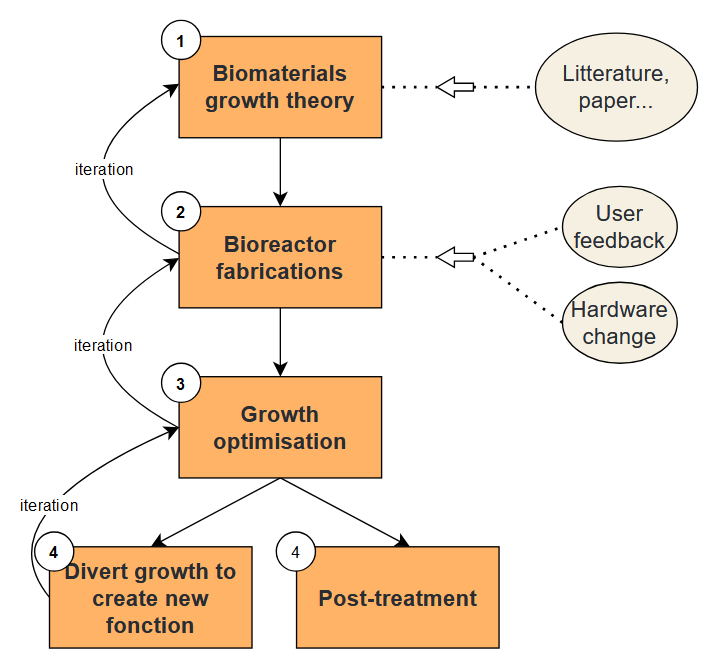
\includegraphics{images/diag_approche.png}
    \caption{General approach overview}
    \label{fig:IS_demo}
\end{figure}


\section{Field of Research}

This research is situated at the intersection of biomaterial science, biological growth processes, and environmental control technologies. Specifically, 
it explores the potential of soft biomaterials such as SCOBY (Symbiotic Culture of Bacteria and Yeast) and mycelium biocomposite, two promising alternatives 
for sustainable material production. 

\paragraph[short]{Biomaterial science} 
Biomaterial science forms the foundation of this research by investigating the properties, applications, and fabrication processes of materials derived from living organisms. 
The study of SCOBY mycelium-based biocomposites is still relatively new, yet early research suggests their high potential for applications in various sectors, including fashion\cite{amobonye2023fungal}, architecture\cite{ghazvinian2019mycelium}, and packaging\cite{abhijith2018sustainable}, where ecological impacts are a growing concern. And as a substitute for certain materials currently derived from fossil resources\cite{jang2017bacterial}.

One of the core aspects of this research is the investigation of the biological growth processes that govern the development of these materials. SCOBY, for instance, grows through a fermentation process where bacteria and yeast work together in a chain reaction where bacteria produce cellulose. Mycelium, on the other hand, forms a dense network of fungal hyphae, which can be molded into various shapes and solid structures. Understanding and optimizing the growth parameters—such as temperature, humidity, and nutrient supply—is essential for ensuring the consistency and quality of the biomaterials produced.

\paragraph[short]{Environmental
control technologies}
To achieve optimal growth conditions, this research integrates IoT-based sensors for real-time monitoring and control of environmental factors within bioreactors. 
The sensors pair with actuator, including temperature, pH, and moisture sensors, provides precise feedback, allowing for the automation of the growth process. 
automation of the growth process. System automation also opens the door to the field of embedded systems and electronics research. 

In the field of plant sciece controlled environment systems, like Phytotron are use to recreate climates to studies plants behavior under experimental conditions.
Unlike Phytotron, the role of the bioreactor is not only to recreate optimal growth conditions, but above all to create specific environmental paramenter or special constrain that allowing the bioreactor to amplify unnatural behavior in order to induce new properties on the biomaterial.  This capability allows for greater customization and the exploration of material innovation, as bioreactors can be programmed to create tailored conditions that go beyond natural biological environments.
 

\paragraph[short]{Low-technologies} 
This thesis also draws inspiration from the philosophy of low-technologies.
Low-technologies offer an alternative to high-tech industrial processes by focusing on accessible, repairable, and sustainable solutions. 
This approach not only reduces environmental impacts but also opens up the possibility for decentralized, small-scale production systems that are adaptable to different geographic and climatic conditions. 
Biomaterials meet this definition, and can be include in lager systems to recycled organic waste as illustration. the low-technologies allready use mycelium biocomposite in in building construction. 

whether it's in the use of biomaterials or in machine design. \textbf{design} is also part of the field of research. particularly in the creation of new imaginary worlds that allow us to glimpse new aesthetics that can influence the way we think about matter. 



\section{Contributions}

The contributions to the field mainly focus on what needs this type of material to be grown and how to optimize it.
It focus on two different types of material. Mycelium and S.C.O.B.Y and their respective bioreactor types. 

The projects focus on the production and use of biomaterials and the manufacture of machines to optimize and automate their development, but also to try to disrupt the natural means of growth or co-design with nature to create new uses or forms for biomaterials thanks to the bioreactor. in ways that go beyond the simple production of raw materials.

The goal was also to develop a methodology to understand and build machine tools in order to develop an approach that can be generalized to other biomaterials.
The Machine also aim to be ergonomic and useful for the final user. Because all this type of machine might be build simply by just using a box and some kind of actuator, the projet aim to show that understand deeply the formation of the biomaterial is an added value if we want to be able to divert the living to make more than raw material or a hight tech greenhouse. 

\chapter{General State of the Art}


\section{Context}

To replace materials that are very practical but very problematic for our environment, convince people of the usefulness of the replacement. on the one hand, by making functional objects. But also by opening the door to new imaginations that broaden the scope of what's possible. that's why, in the same way as classical research, design helps to shape this problem. 
\begin{marginfigure}[-5cm] % Adjust the vertical placement
    \centering
    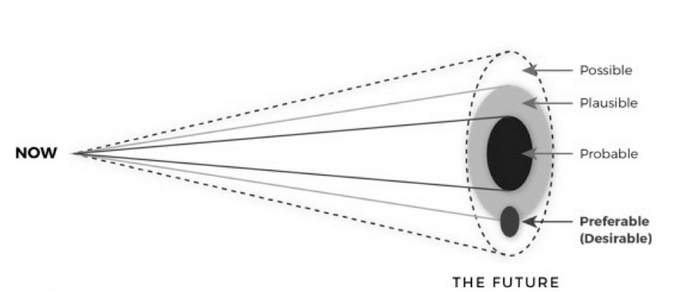
\includegraphics[width=\linewidth]{images/futures_cone.png}
    \caption{futures cone representation}
    \label{fig:plastics}
\end{marginfigure}
Science in this field relatively new. The starting point differs depending on how define biomaterials and how make, or rather grow them. 
More globally, biomaterials are at the crossroads of many fields of scientific and even artistic research. From agriculture to design, from synthetic biology to fashion, from DIY fermented drink to biohacking in the kintchen\cite{CiteTheOdin}.
This is in line with new interdisciplinary courses integrating biodesign, such as MIT's "How To Grow (Almost) Anything" course\cite{CiteMITHTGAA}. 

As matter of fact, the starting point might be the first crops domestication. At this time the goal was only to produce food, and the process were optimized by selective breeding. By taking the plants with the biggest fruit or the best resistance to environment, from generation to generation plants were "optimized" for the population.
Besides, the use of wood are very use in numerous sectors\cite{ramage2017wood} push by international directive of less CO2 emmission and waste. 
  
However, today, biomaterials or biobased materials in this study are more in line with the aim of replace existing materials like plastics.
This biomaterials production projects are aimed to create in the futures of cone plausible or possible futures. 
Moreover the development of this new materials go hand in hand with the evolution of new machines for biomaterials. Bioreactors are controlled environment systems. There is no notable differences in hardware part from bioreactors in the litterature. The general form is a isolated space from outside environmental conditions, 
combine with a controler responsible of sensors and actuator (i.e :fogger, fan, thermal resistance...). The controler is also responsible to send data when monitoring is wanted. All powered by energy from different sources. 

Multiple reviews\cite{cottet2020biobased}\cite{vinod2020renewable}\cite{hairon2022bio} about biobased materials support for the fact that today's synthetic materials, especially those derived from oil, are a problem for human and ecosystem health.
These studies reveals the strong interess of these materials in term of sustainability and low cost production, and "by reducing wastages, landfills
and toxic emissions leading to greener and cleaner environment". They also show end proprieties these materials are distinguished by their biodegradability and compostability. Which also makes them interesting for their end-of-life properties. 
However, there are concers about a lack of large scale industrialisation and a lack standadise methodology \cite{andrew2022sustainable}. This leads to a lack of confidence in mechanical properties, as the absence of standardization, give rise to the limited exploitation of technical data on characteristics such as tensile strength, compression, fatigue, impact resistance and flammability, makes assessment more difficult.   
Into the bargain, most of these materials are and highly anisotropic.

\paragraph[short]{Industry} 
Ecovative and MycoWorks lead in mycelium-based biomaterials. Ecovative creates eco-friendly alternatives to plastics for packaging and construction, while MycoWorks focuses on sustainable mycelium leather, targeting fashion and luxury markets.
\paragraph[short]{In Design} 
Suzanne Lee, through Biofabricate, pioneers biofabrication in design, using biological processes to grow sustainable materials like microbial leather, pushing the boundaries of traditional manufacturing and eco-conscious design.


\section{Biomaterial}
\subsection{S.C.O.B.Y Lether} 

\paragraph[short]{Definition } 
S.C.O.B.Y, aim to Symbiotic Culture Of Bacteria and Yeast, during this symbiotic culture a lot of biochimical element are tranformed or exchanged by bacteria and yeast.
Among this biochimical elements, there is bacterial cellulose. Bacterial cellulose(BC) is a biopolymer that grows on the surface of the culture medium. 

More precisely, 2 metabolic processes are at play, in a kind of “double” fermentation. 
on the one hand, alkolic fermentation by leaven. In other words, the glucoses will be converted into ehtanol. 
on the other hand, “acetic fermentation” by bacteria. In other words, the ethanol will be converted into acetic acid.

C_6H_{12}O_6 + 2 \, \text{ADP} + 2 \, P_i \rightarrow 2 \, \text{ATP} + 2 \, H_2O + 2 \, CH_3CH_2OH + 2 \, CO_2

CH_3CH_2OH + O_2 \rightarrow CH_3COOH + H_2O

in addition to the metabolic processes that allow these microorganisms to survive and reproduce, bacteria will also synthesize this so-called bacterial cellulose.




\paragraph[short]{Use}

\subsection{Mycelium}


\subsection{Other Biomaterial}




















\section{Bioreactor \& Controlled Environment }

\subsection{Controlled Environment} 



















\subsection{Bioreactor}
\subsection{Bioreactor S.C.O.B.Y}
\subsection{Bioreactor Mycelium}



\section{Discution and limitation}
\chapter{Mycelium Machine \& Materials}


\section{Overview}

This projects aim to develop an easy way to make mycelium-based biocompisites. We present two similar Controlled Environment systems for mycelium based composite that can be developed easily with DIY and low cost hardware.
One of this project focus more on monitoring un data management, the other one is mare about modularity and transport 
In both cases, we're talking about controlled-environment systems with a closed space, thermal resistance or heating mats, temperature sensors, humidity modulators and associated relative humidity sensors, carbon dioxide sensors and fans for air renewal and circulation. 
And of course a control and data transmission system. 

% \begin{figure}[h]
%     \centering
%     \includegraphics{images/Myceliummachine.png}
%     \caption{System design representation}
%     \label{fig:}
% \end{figure} 

\section{Systems design}

The controlled Environment systems takes the form of a closed box, isolated from external climatic conditions. this box is where the inoculated substrate for mycelium growth is placed: “Mycelium grow space”. 
The Mycelium grow space is instrumented with climate sensors. in this case a relative humidity sensor, a temperature sensor and a carbon dioxide sensor. they are connected to an ESP-type microcontroller which handles data reading.
The ESP will then send the data via an MQTT protocol to a RaspberryPI acting as an MQTT broker and server for an Influx database. The data can then be visualized via a dashboard on a user's computer. 

On the ESP, a main user can select the desired climate variables. This will change the conditions according to which the microcontroller will activate or deactivate relays. This will switch on or off climatic actuators (ie: thermal resistance etc...) which will also change the internal climatic conditions in the space.  
Everything will act automatically once the variables have been chosen by the user (Automation loop). 

This architecture allows the simultaneous use of several controlled environments with different growth conditions. Users can choose, via the MQTT protocol, whether or not to subscribe to a controlled environment and see the data associated with it. 

\begin{figure}[h]
    \centering
    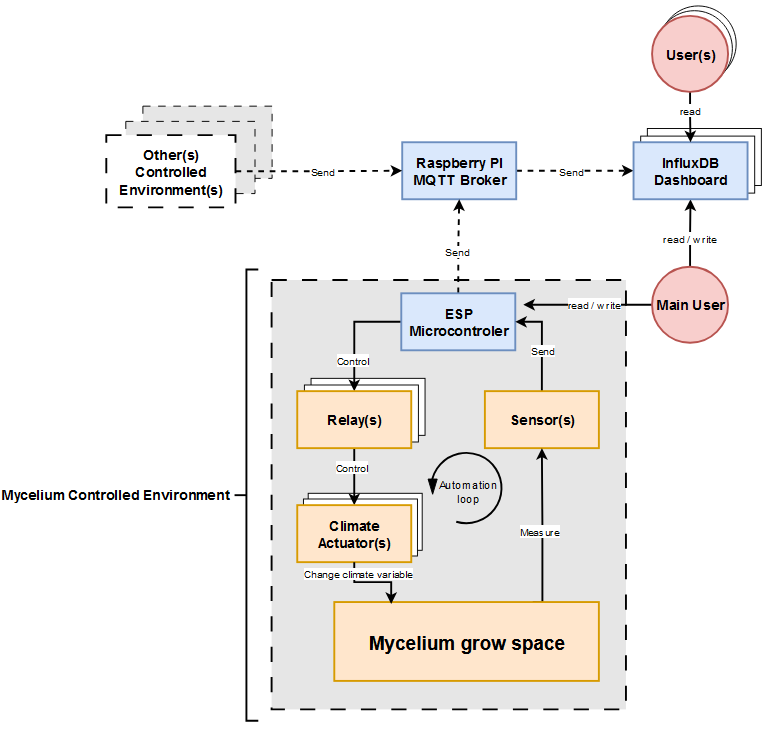
\includegraphics[width=1.4\textwidth]{images/diagMyceliummachine2.png}
    \caption{System design representation}
    \label{fig:blasttrash}
\end{figure} 


\section{Manufacturing Processes \& Grow Theory}

In a natural environment, the mycelium grows in the soil in search of nutrients. when it emerges from the soil into the air or under leaves, it is still in an environment rich in carbon dioxide. at this point, the mushroom stem (fruit of the mycelium) will grow until it reaches the air with more oxygen and forms the mushroom cap. 

In the case of Mycelium-based biocomposite, the mycelium will be innoculated in a substrate rich in nutrients and/or fibrous material. 

As explained above, the mycelium will agglomerate the substrate, greatly increasing the solidity of the innoculated substrate compared with the solidity prior to growth. 
When the mycelium comes into contact with the substrate in an oxygen-rich environment, it will blach and form a hydrophobic, fireproof layer.
That is why control carbon dioxide concentration is very important for mycelium material

Air renewal is also important for two other reasons: on the one hand, mushrooms breathe like we do, so they consume oxygen and spit out carbon dioxide. So the carbon dioxide concentration in the closed enclosure increases over time. Without air renewal, the mycelium will eventually aphyxiate itself. 
On the other hand, air renewal reduces the appearance and development of other pathogens or molds that would compete with the mycelium, and thus reduce its development. 


\paragraph[short]{Manufacturin Processes}

The approach is very similar to the literature described above \ref{Fab_process}.
first, the substrate is sterilized. then mycelium is mixed with the substrate in molds and placed in the controlled Environment for two or three weeks. 

During growth, once the mycelium has grown enough that the inoculated substrate no longer needs to be in the mold for growth. 
Then the molds are carefully removed to allow the mycelium to breathe as much as possible, especially on the surfaces in contact with the mold. 

After the growing phase, the Mycelim based biocompisites are dried in an oven for a minimum of 5 hours, depending on size or thickness, at a maximum of 80°C. 

\section{Contribution}

\subsection{Environment controlled}

The project consists of 3 main sections: the mycelium growth area, the water tank and the electrical panel.

The mycelium-growing part is a plastic box of around 100 liters, with its walls lined with bubble-wrap to provide thermal and light insulation. The box has also been modified by adding elastics to create tiers in the box to accommodate the molds and ensure uniform air circulation. The box houses the sensors directly connected to the electric panel and also houses thermal resistance. This section has 3 pipes. 2 for the air inlet and outlet sent by the filter fans, and one connected to the water tank.

The water tank consists of a water box containing a fogger and a centrifugal fan, both of which are connected to the electrical panel. There is an air inlet and an air outlet. The fan is located at the air inlet, while the air outlet is connected by a pipe to the growth space.

The fogger is immersed in the water in the reservoir. When the fogger and fan are switched on, the fogger will create an aerosol of water which will be transported to the growth space via the air flow created by the fan. This will increase the humidity in the growth space.

The electrical panel manages all the electrical or electronic parts of the project. In other words, the power supply, the microcontroller and the relays that control the various climatic actuators. The electrical panel is connected via a mains socket to power the entire system.

Everything was placed on a large board overlaid with wheels for ease of movement. 
% \begin{figure}[h]
%     \centering
%     \includegraphics{images/Myceliummachine.png}
%     \caption{System design representation}
%     \label{fig:}
% \end{figure} 


The mycelium used was ganoderma lucidum, also known as reishi, the most widely used mushroom in the literature.\cite{yang2021material}
Moreover, this mushroom seems to have better mechanical properties, even if it seems that it's mainly the subtrate that dominates over the mechanical properties. 

Several types of substrate have been tested. More fibrous substrates such as coconut fiber. More granular substrates such as corn husks. Nutrient-rich substrates such as coffee grounds. Low-organic substrates composed mainly of minerals. 
And combination mixes of its substrates.

In addition, the direction of the fibers in the substrate also affects the mechanical properties. In other word fibrous substrates may have greater mechanical properties or the opposite, depending on how they were placed in the substrate.


\subsection{Modular environmental control}

This design is quite different from the contolled environment presented just before. 
The aim here is to present an easy way of unpacking a controlled environment. Firstly, the system can be completely dismantled to take up as little space as possible. 

The 3 sections presented above (I.e : the mycelium growth area, the water tank and the electrical panel.) are also found in this system to perform the same functions, but they have different characteristics.

The mycelium growth area,consists of a parallelepiped formed by aluminum profiles for the edges and cushions made from 2 sheets of transparent PVC for the faces. The cushions are inflated with air to provide better thermal insulation. These faces are fixed to the aluminum profile via velco tape. The top and bottom faces (the smallest faces) are in plexiglass. 

This is the part that takes up the most space in traditional designs. Here, all the growth  space is removable. The PVC sides can be deflated and then folded. The aluminum profiles can be removed to take up less space.

The equivalent of the electrical panel is located under the growth space in a small space in an MDF box where the electronics and power supply are located. There are several cables running in and out of this section the main power cable and the power supplies for the sensors and climatic actuators except for the fogger. Inside this hole are the relays and the microcontroller. 

The second special feature of this system is that the water reservoir and the fogger are not located close to the system, but are connected to it by a pipe. The water reservoir constantly generates water aerosol, and humidity is supplied via a fan in the growth space. 
Which makes it easy to centralize several contrasting environments around the tank for testing different cliamatic variables at the same time. 

%%%%%% photo avant apres demontage 
photo avant apres demontage ???????









\section{Result}
\subsection{Mechanical test}



\chapter{SCOBY Machine \& Materials}


\section{Overview}

In the same way as for the environent control project with the scoby, we had to think about how machines can help us make this new material our own, in much the same way as 3D printers popularized the use of PLA. 

The methods and machines presented here are designed to facilitate the use of this biomaterial, with the aim of optimizing the production of bacterial cellulose and changing the growing conditions to produce 3D cellulose. 

In addition, unlike mycelium, which unfolds in a substrate contained in a mold, cellulose requires more attention to shape channelling, both for molding and demolding. 

\begin{figure}[h]
    \centering
    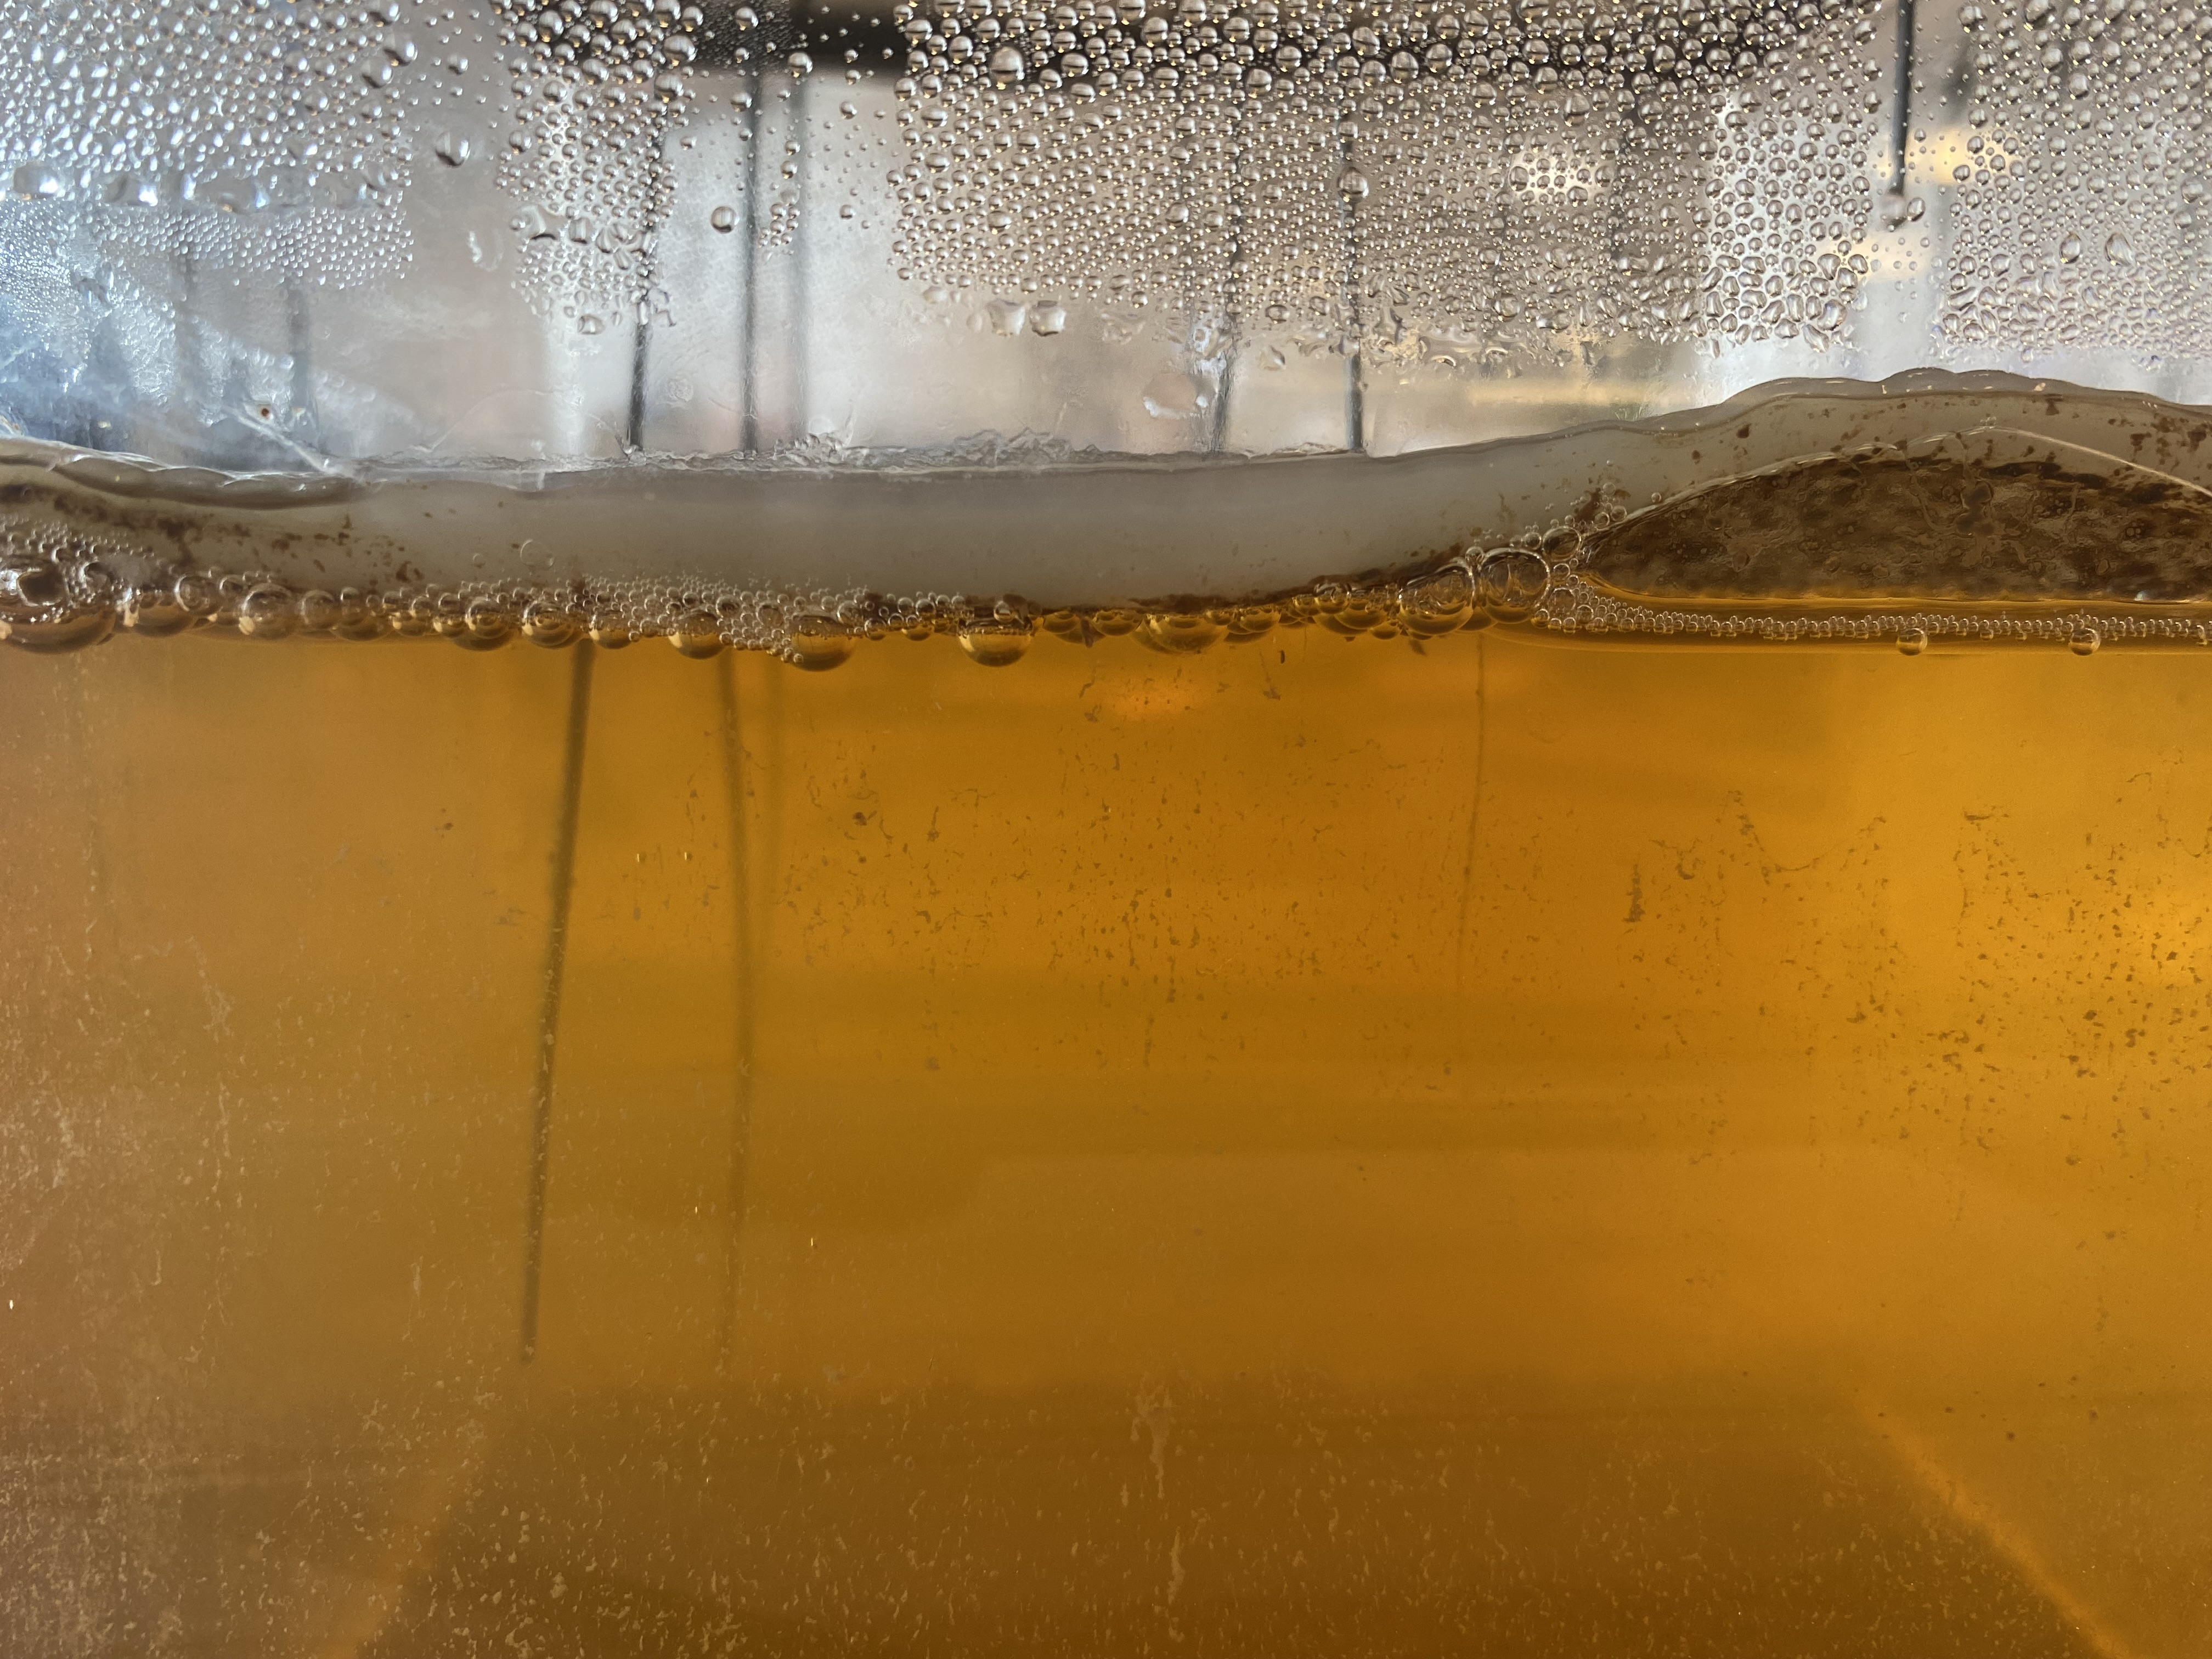
\includegraphics{images/IMG_4126.jpg}
    \caption{Bacterial cellulose at the sufface and it meidium}
    \label{fig:}
\end{figure} 

\section{Systems design}


In the traditional approach, cellulose grows on the surface of the liquid, which means that the cellulose takes on a flat shape \- the shape of the container in which the bacterial cellulose grows. 

With the bioreactor, there are two objectives. on the one hand, to optimize production. On the other hand, to modify the natural growth of poccesus in order to be able to make more complex shapes than 2D shapes. 

To achieve this, the method used is to introduce a 3D shape that rotates on the surface of the liquid so that the cellulose can adhere to the shape and push against it. As shown in the following diagram. 

the bioreactor incorporates a rotating framework, typically shaped to encourage cellulose attachment and buildup in desired forms beyond a simple flat surface. This framework is submerged in a controlled culture medium, allowing the bacteria to deposit cellulose around a defined 3D scaffold as it rotates. The rotation ensures even cellulose distribution, encouraging layers to adhere around the object and gradually form into three-dimensional shapes.
\begin{figure}[h]
    \centering
    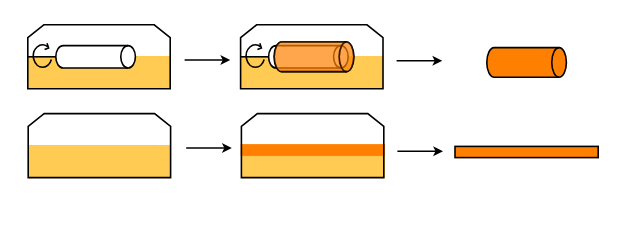
\includegraphics{images/shema3Dscoby.png}
    \caption{System design representation for 3D bacterial cellulose}
    \label{fig:diagBC3D}
\end{figure} 

The bioreactor takes the form of a closed space like a box, with openings covered with microporous plaster to allow air to pass through without contaminating the space. Into which the culture medium can be introduced.
It is generally located in a closed space in which a heating mat is installed to maintain a suitable temperature for better cellulose development. 
heating mat helps sustain an optimal temperature for bacterial activity, while microporous openings enable airflow, preventing contamination while ensuring that the bacteria have sufficient oxygen. Adjusting rotation speed and environmental factors enables control over cellulose thickness.


\section{Manufacturing Processes \& Grow Theory}


\begin{figure}[h]
    \centering
    \includegraphics[width=0.7\textwidth]{images/prodperso.png}
    \caption{Bacterial cellulose after growth period}
    \label{fig:manufactureperso}
\end{figure} 

In kombucha production, bacterial cellulose naturally forms a film on the surface of the liquid medium. The Acetobacter bacteria in the SCOBY (Symbiotic Culture of Bacteria and Yeast) convert sugars in the medium into long cellulose fibers when exposed to oxygen. This fibrous structure gradually accumulates, forming a thick cellulose layer that acts as a barrier, potentially preventing other microorganisms from entering the medium. The cellulose matrix produced this way is thought to provide protection for the bacteria by limiting microbial competition.

This cellulose production process operates from the top of the solution downward. As cellulose accumulates, the older layers sink, leaving the most recently formed cellulose on the top surface exposed to oxygen. This layered formation is key to producing thick, multi-layered sheets of cellulose that can later be harvested.

The process of creating bacterial cellulose involves two main stages: preparing the culture medium and setting up the bioreactor. In preparing a homemade culture medium, freshly crushed bacterial cellulose is added to a nutrient solution composed of tea, water, sugar, and a small amount of vinegar to maintain an acidic environment conducive to bacterial growth.

\-- Boil the Water: This step sterilizes the water and allows the tea to fully infuse.

\-- Add Tea, Sugar, and Vinegar: These elements provide essential nutrients. The tea provides nitrogen, while sugar is the primary energy source for the bacteria. Vinegar lowers the pH, creating a favorable acidic environment.

\-- Cool the Solution: Allow the mixture to cool below 30°C to avoid harming the living cultures.

\-- Introduce Crushed Cellulose: Adding bacterial cellulose from an older culture introduces live bacterial strains to kickstart the cellulose production.

\begin{figure}[h]
    \centering
    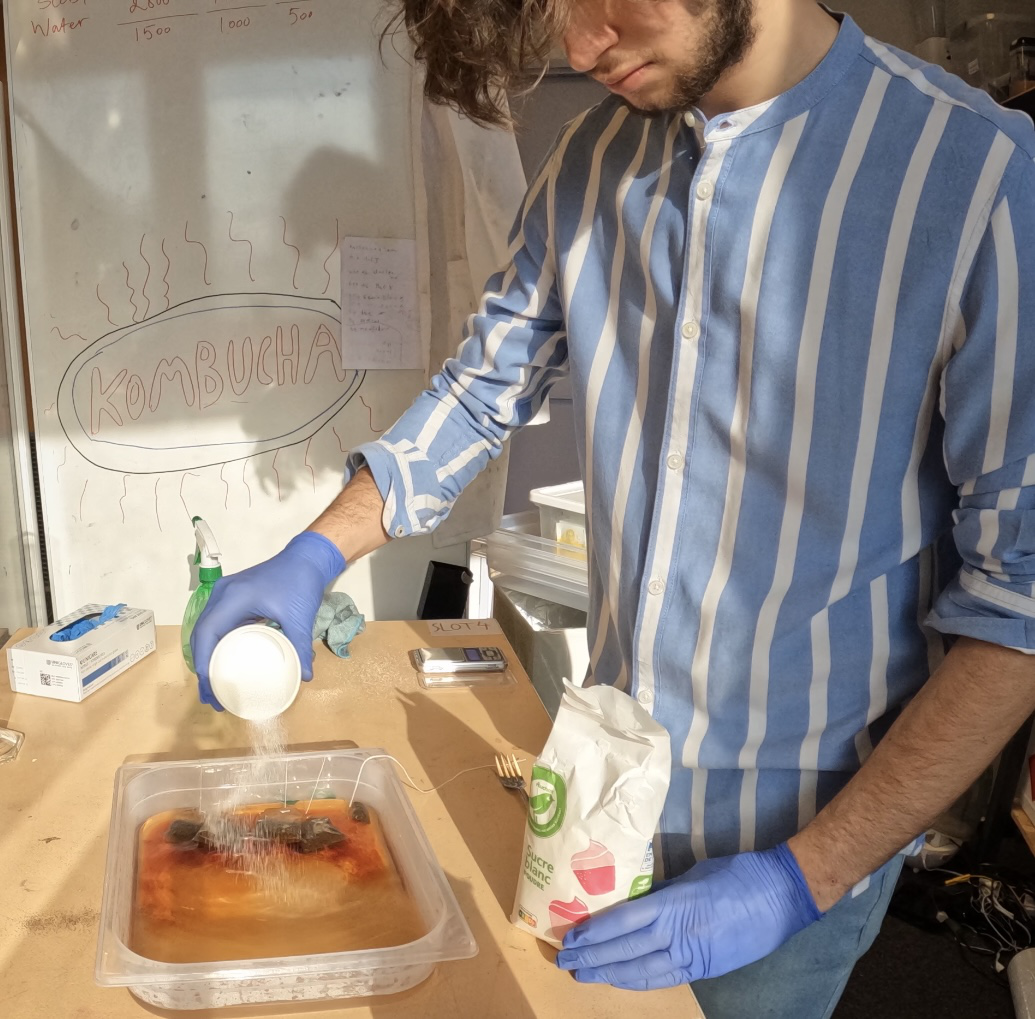
\includegraphics[width=0.7\textwidth]{images/preparation.png}
    \caption{preparation of medium}
    \label{fig:manufactureperso2}
\end{figure} 
Once the medium is prepared, it is transferred into a bioreactor, typically a container that promotes even growth. After approximately 14 days, a cellulose mat forms on the surface. This mat is then harvested, and the process can be repeated to cultivate a cellulose strain optimized for desired growth characteristics.

\begin{figure}[h]
    \centering
    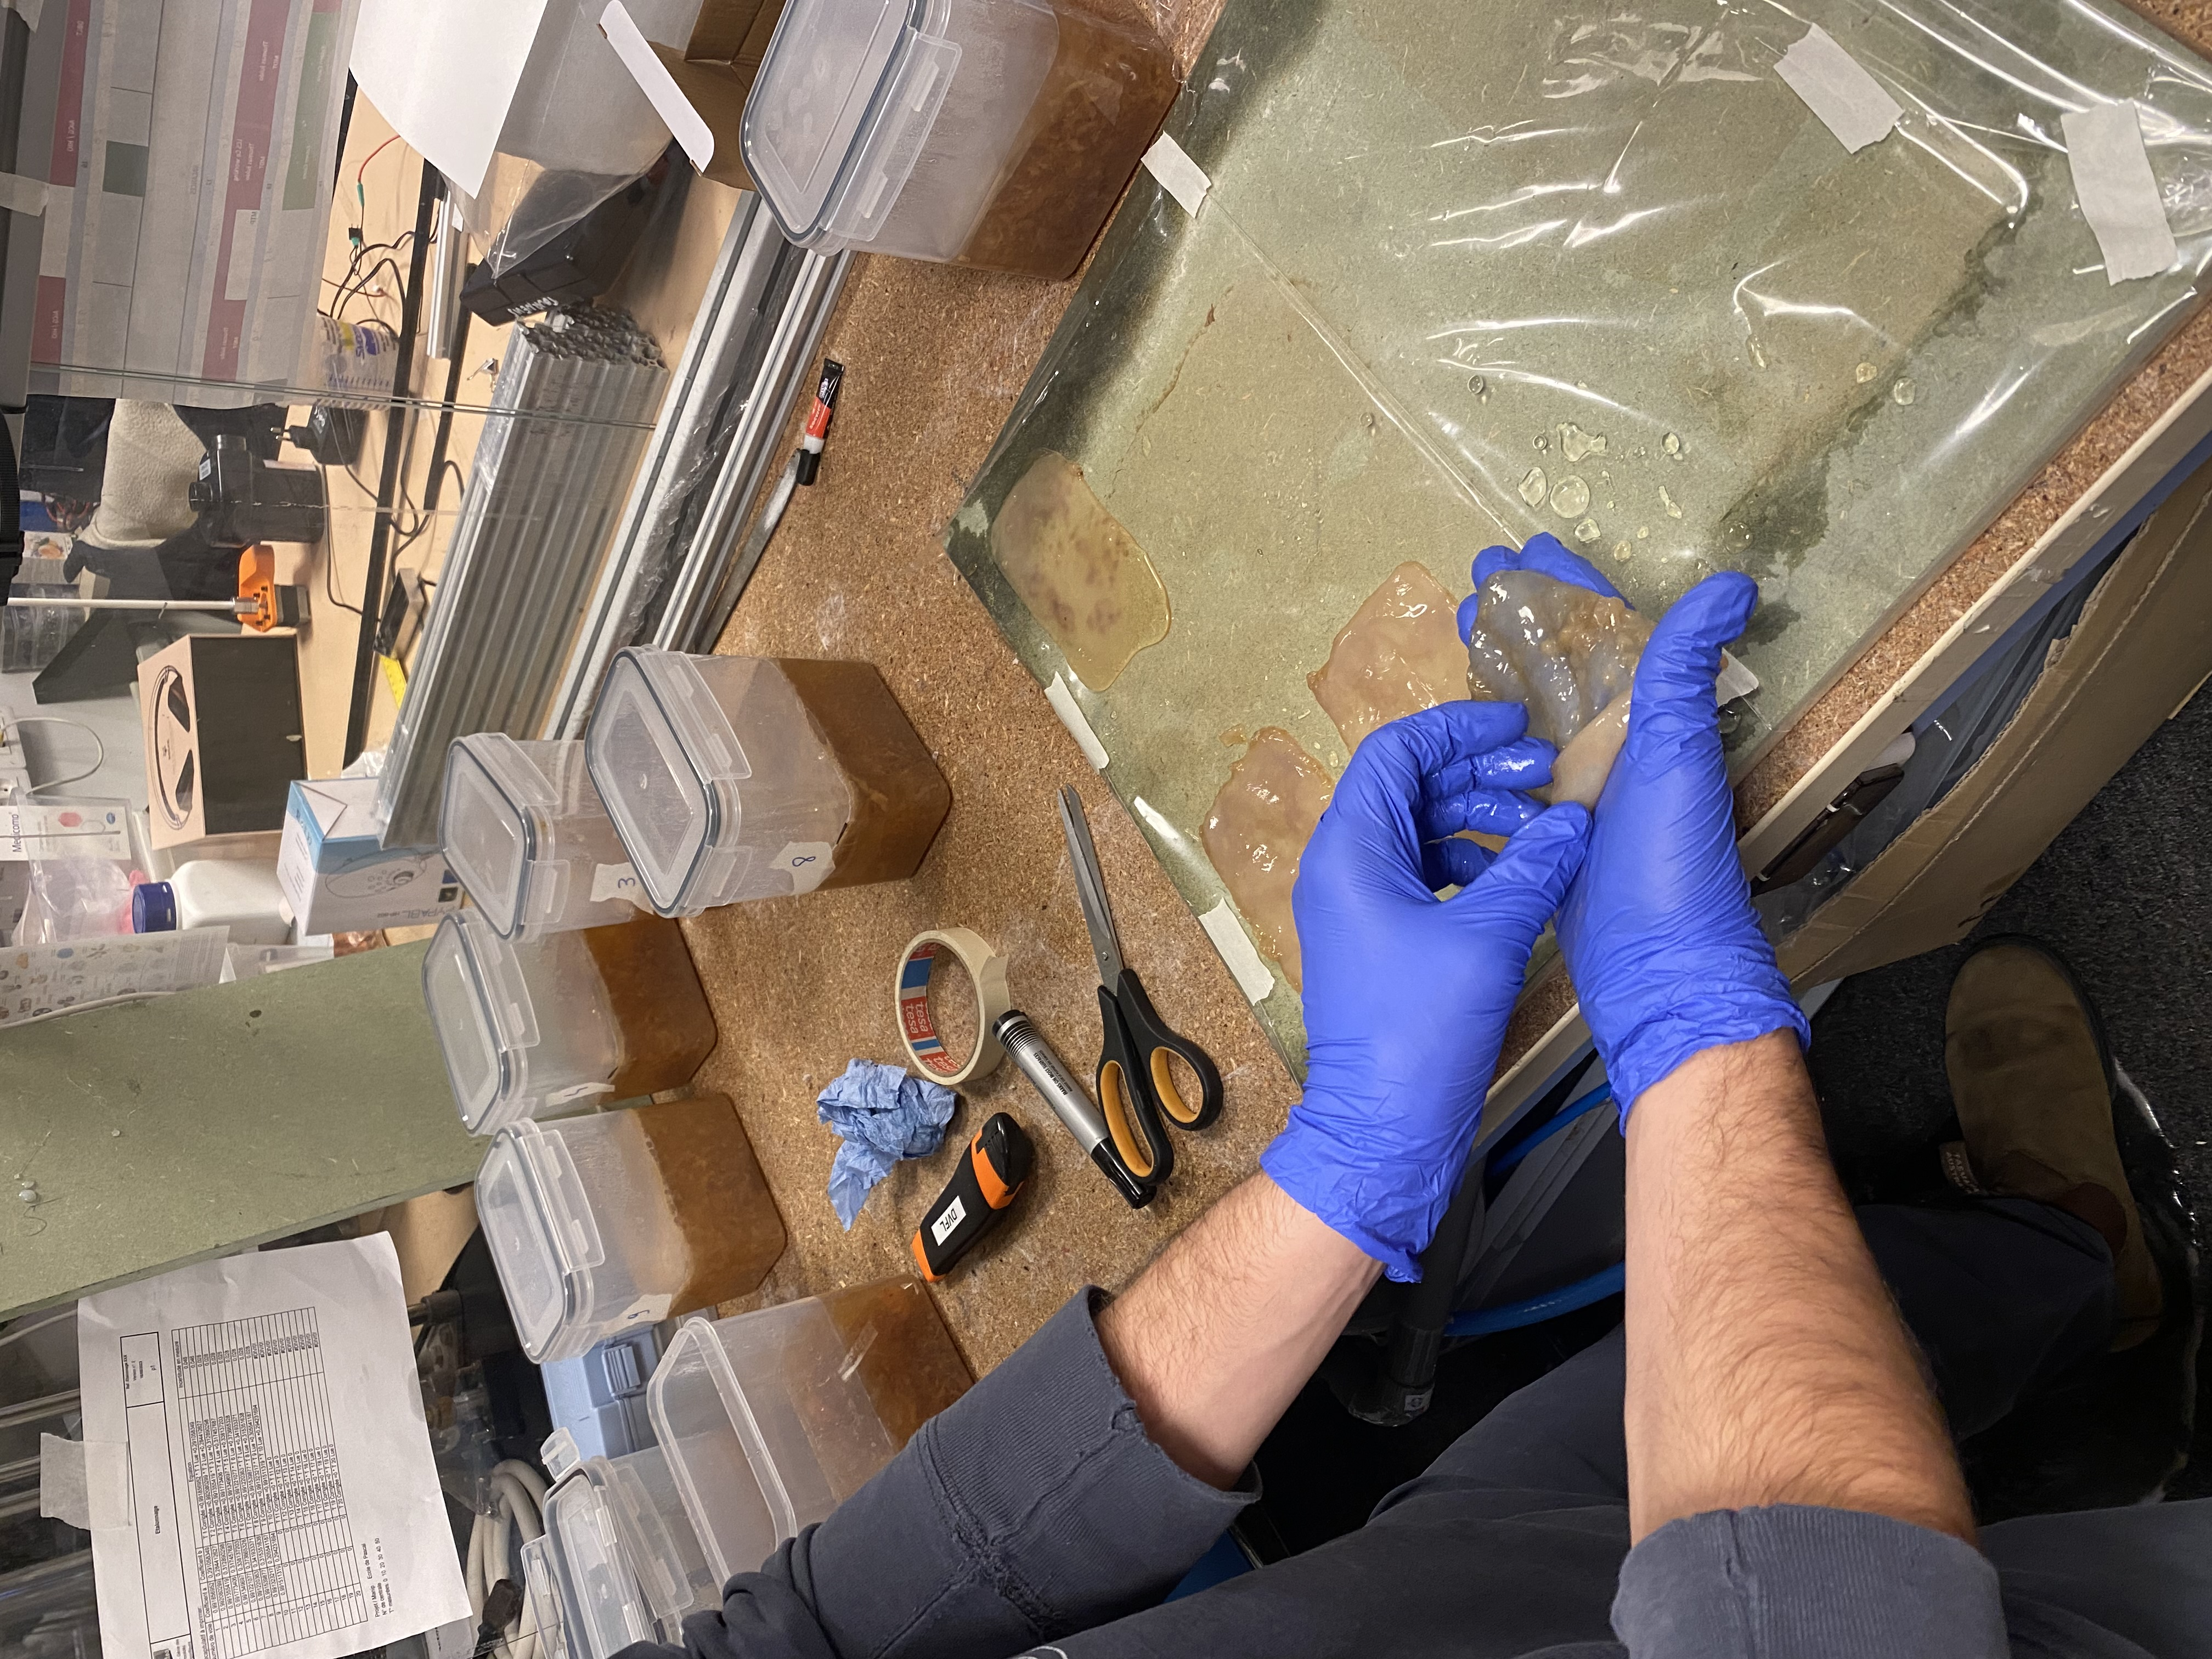
\includegraphics[width=0.7\textwidth]{images/IMG_4565.jpg}
    \caption{preparation of cellulose before drying process}
    \label{fig:manufactureperso3c}
\end{figure} 
Drying and Final Processing: After growth, the cellulose mat is carefully removed and dried to achieve its final texture and strength. The drying process removes about 90\% of its water content, reducing the cellulose sheet to its final shape and thickness, making it durable and ready for various applications.



\begin{figure}[h]
    \centering
    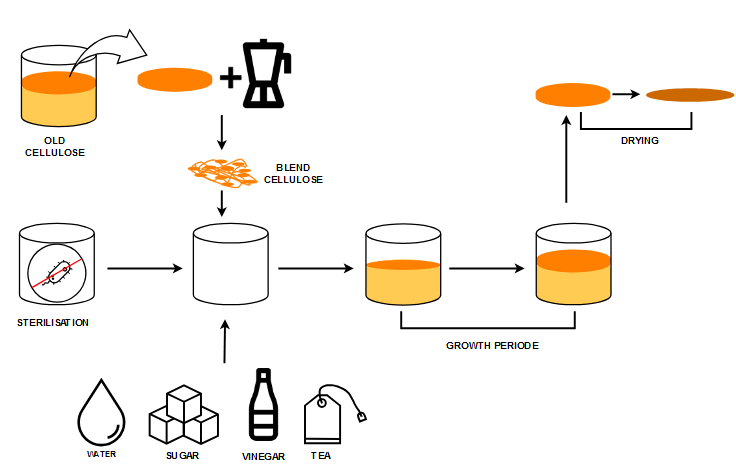
\includegraphics[width=1.2\textwidth]{images/SCOBY_diag.png}
    \caption{Classical manufacturing processes}
    \label{fig:manufacture}
\end{figure} 

\section{Contribution}

\subsection{Rotary Bioreactor}
The project consists of a rather unusual bioreactor. The bioreactor is made up of two closed enclosures, one inside the other.

In the larger of the two, there's a heating mat to raise the temperature for faster cellulose development, and a motor with a transmission system that turns a shaft in the smaller chamber. It's in the smaller one that the growing medium will be located.

In this configuration, the cellulose will not grow on the surface but on the shape in question, which will form cellulose in 3 dimensions with the shape of the surface of the shape on the axis. 

This innovative bioreactor configuration is designed to overcome the traditional limitations of bacterial cellulose growth, which typically forms flat sheets on the surface of the liquid medium. By introducing a rotating axis and shaping system, this bioreactor enables the cultivation of cellulose in three dimensions, opening the door to new applications and geometries.

The smaller, internal chamber serves as the primary growth environment. Here, the shape to be coated in cellulose is mounted onto the rotating shaft, allowing it to continually move through the culture medium. This rotation ensures even exposure of the shape to the bacteria and nutrients, promoting uniform cellulose deposition across its surface. The movement also helps disrupt stagnation zones, improving nutrient distribution and oxygen exposure to support optimal bacterial activity.

The larger, external chamber acts as a controlled environment for the process. The heating mat is essential for maintaining an ideal temperature, typically around 25–30°C, which accelerates bacterial cellulose synthesis without compromising quality. The bioreactor's design also incorporates ventilation with microporous filters to allow oxygen exchange while preventing contamination. This ensures the bacterial culture remains healthy and active throughout the production cycle.

This method allows for precise control over the final product's geometry, enabling the creation of hollow structures, complex curves, and other intricate forms not possible with traditional surface-grown cellulose. 
\begin{figure}[h]
    \centering
    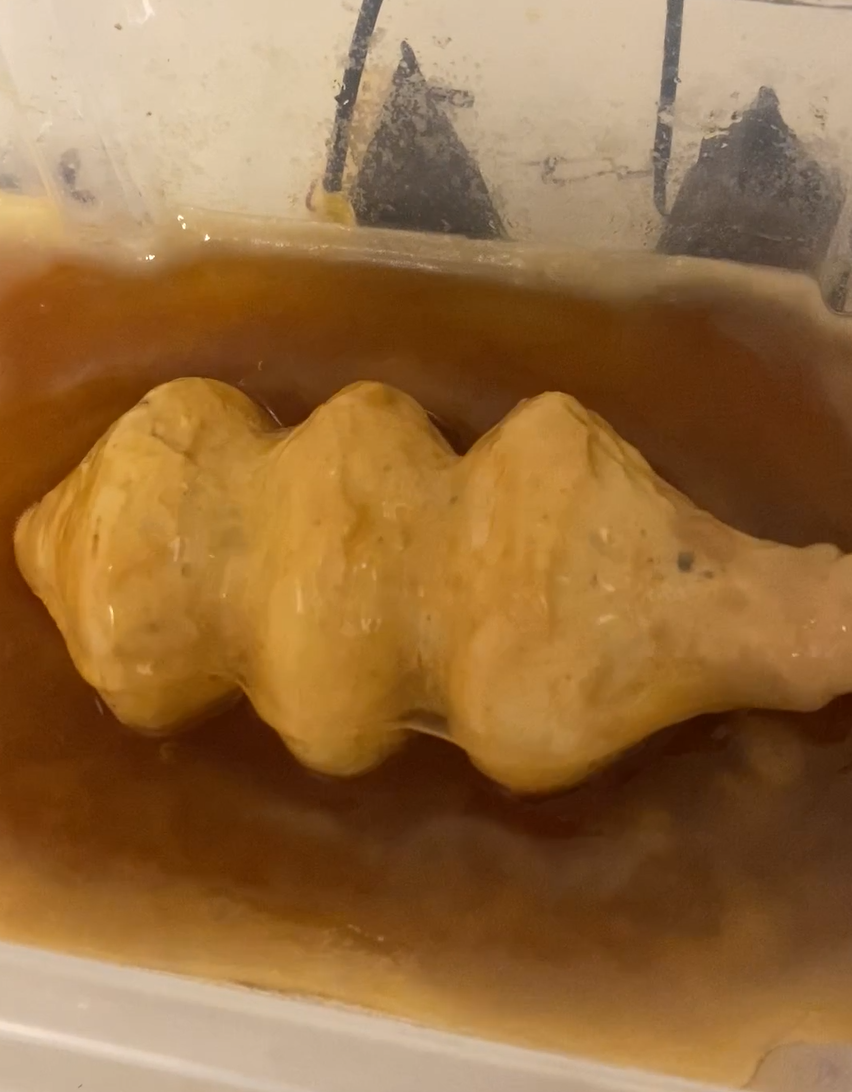
\includegraphics{images/insiderotary.png}
    \caption{Inside grow culture medium on rotary bioreactor}
    \label{fig:rotary inside}
\end{figure} 

\section{Result}

\subsection{traditional approach}

\subsection{rotary approach}
\chapter{Conclusion}



%----------------------------------------------------------------------------------------

\backmatter % Denotes the end of the main document content
\setchapterstyle{plain} % Output plain chapters from this point onwards

%----------------------------------------------------------------------------------------
%	BIBLIOGRAPHY
%----------------------------------------------------------------------------------------

% The bibliography needs to be compiled with biber using your LaTeX editor, or on the command line with 'biber main' from the template directory

\defbibnote{bibnote}{Here are the references in citation order.\par\bigskip} % Prepend this text to the bibliography
\printbibliography[heading=bibintoc, title=References, prenote=bibnote] % Add the bibliography heading to the ToC, set the title of the bibliography and output the bibliography note

%----------------------------------------------------------------------------------------
%	NOMENCLATURE
%----------------------------------------------------------------------------------------

% The nomenclature needs to be compiled on the command line with 'makeindex main.nlo -s nomencl.ist -o main.nls' from the template directory

% \nomenclature{$c$}{Speed of light in a vacuum inertial frame}
% \nomenclature{$h$}{Planck constant}

% \renewcommand{\nomname}{Notation} % Rename the default 'Nomenclature'
% \renewcommand{\nompreamble}{The next list describes several symbols that will be later used within the body of the document.} % Prepend this text to the nomenclature

% \printnomenclature % Output the nomenclature

%----------------------------------------------------------------------------------------
%	GREEK ALPHABET
% 	Originally from https://gitlab.com/jim.hefferon/linear-algebra
%----------------------------------------------------------------------------------------

% \vspace{1cm}

% {\usekomafont{chapter}Greek Letters with Pronounciation} \\[2ex]
% \begin{center}
% 	\newcommand{\pronounced}[1]{\hspace*{.2em}\small\textit{#1}}
% 	\begin{tabular}{l l @{\hspace*{3em}} l l}
% 		\toprule
% 		Character & Name & Character & Name \\ 
% 		\midrule
% 		$\alpha$ & alpha \pronounced{AL-fuh} & $\nu$ & nu \pronounced{NEW} \\
% 		$\beta$ & beta \pronounced{BAY-tuh} & $\xi$, $\Xi$ & xi \pronounced{KSIGH} \\ 
% 		$\gamma$, $\Gamma$ & gamma \pronounced{GAM-muh} & o & omicron \pronounced{OM-uh-CRON} \\
% 		$\delta$, $\Delta$ & delta \pronounced{DEL-tuh} & $\pi$, $\Pi$ & pi \pronounced{PIE} \\
% 		$\epsilon$ & epsilon \pronounced{EP-suh-lon} & $\rho$ & rho \pronounced{ROW} \\
% 		$\zeta$ & zeta \pronounced{ZAY-tuh} & $\sigma$, $\Sigma$ & sigma \pronounced{SIG-muh} \\
% 		$\eta$ & eta \pronounced{AY-tuh} & $\tau$ & tau \pronounced{TOW (as in cow)} \\
% 		$\theta$, $\Theta$ & theta \pronounced{THAY-tuh} & $\upsilon$, $\Upsilon$ & upsilon \pronounced{OOP-suh-LON} \\
% 		$\iota$ & iota \pronounced{eye-OH-tuh} & $\phi$, $\Phi$ & phi \pronounced{FEE, or FI (as in hi)} \\
% 		$\kappa$ & kappa \pronounced{KAP-uh} & $\chi$ & chi \pronounced{KI (as in hi)} \\
% 		$\lambda$, $\Lambda$ & lambda \pronounced{LAM-duh} & $\psi$, $\Psi$ & psi \pronounced{SIGH, or PSIGH} \\
% 		$\mu$ & mu \pronounced{MEW} & $\omega$, $\Omega$ & omega \pronounced{oh-MAY-guh} \\
% 		\bottomrule
% 	\end{tabular} \\[1.5ex]
% 	Capitals shown are the ones that differ from Roman capitals.
% \end{center}

%----------------------------------------------------------------------------------------
%	GLOSSARY
%----------------------------------------------------------------------------------------

% The glossary needs to be compiled on the command line with 'makeglossaries main' from the template directory

% \newglossaryentry{computer}{
% 	name=computer,
% 	description={is a programmable machine that receives input, stores and manipulates data, and provides output in a useful format}
% }

% Glossary entries (used in text with e.g. \acrfull{fpsLabel} or \acrshort{fpsLabel})
\newacronym[longplural={Frames per Second}]{fpsLabel}{FPS}{Frame per Second}
\newacronym[longplural={Tables of Contents}]{tocLabel}{TOC}{Table of Contents}

\setglossarystyle{listgroup} % Set the style of the glossary (see https://en.wikibooks.org/wiki/LaTeX/Glossary for a reference)
\printglossary[title=Special Terms, toctitle=List of Terms] % Output the glossary, 'title' is the chapter heading for the glossary, toctitle is the table of contents heading

%----------------------------------------------------------------------------------------
%	INDEX
%----------------------------------------------------------------------------------------

% The index needs to be compiled on the command line with 'makeindex main' from the template directory

\printindex % Output the index

%----------------------------------------------------------------------------------------
%	BACK COVER
%----------------------------------------------------------------------------------------

% If you have a PDF/image file that you want to use as a back cover, uncomment the following lines

%\clearpage
%\thispagestyle{empty}
%\null%
%\clearpage
%\includepdf{cover-back.pdf}

%----------------------------------------------------------------------------------------
%\usepackage{marginnote}
%\usepackage{sidenotes} % Load the sidenotes package if not already loaded

%\usepackage{afterpage}

% \newcommand\blankpage{%
%     \null
%     \thispagestyle{empty}%
%     %\addtocounter{page}{-1}%
%     \newpage}



\end{document}
